\documentclass{beamer}

\beamertemplatenavigationsymbolsempty

\usepackage[utf8]{inputenc}
\usepackage{listings}
\usepackage{minted}
\usepackage{tikz}
\usepackage{algorithmic}

\usetikzlibrary{graphs,quotes,arrows.meta}
\definecolor{themegreen}{RGB}{0,100,0}
\definecolor{themelightgreen}{RGB}{230,239,230}
\definecolor{themelightblue}{RGB}{215,215,240}

\tikzset{
  pics/square/.default={1},
  pics/square/.style = {
    code = {
    \draw[pic actions] (0,0) rectangle (#1,#1);
    }
  }
}

% set graphics path to figure
\graphicspath{{./figures/}}

\usetheme{Madrid}
\usecolortheme{seahorse}
%Information to be included in the title page:
\title[DataFlowTasks] % optional short title
{DataFlowTasks.jl}

% Custom commands
\newcommand{\DFT}{\texttt{DataFlowTasks.jl}}

\subtitle{Julia \texttt{Task}s which automatically handle data-dependencies}

\author[Faria, Févotte] % short version of authors
{Luiz~M.~Faria\inst{1} \and François Févotte\inst{2}}

\institute[]
{
    \inst{1}%
    Research scientist\\
    INRIA
    \and
    \inst{2}%
    Chief Scientist\\
    TriScale innov
}

\AtBeginSection[]
{
    \begin{frame}
        \frametitle{Table of Contents}
        \tableofcontents[currentsection]
    \end{frame}
}

\date{JuliaCon Local Eindhoven\\December 1, 2023}

\titlegraphic{
  \includegraphics[height=0.5cm]{inr_logo_rouge.png}\hspace{2em}
  \includegraphics[height=0.5cm]{poems_logo.png}\hspace{2em}
  \includegraphics[height=0.5cm]{triscale_couleur_texteadroite.png}
}

\begin{document}

\frame{\titlepage}

% small textsize on frame
\begin{frame}[fragile]
\frametitle{Overview}

\begin{itemize}
    \item \DFT{} is a Julia package dedicated to parallel programming on
      \textit{\textbf{multi-core shared memory CPUs}}.
    \item Automatically infer \texttt{Task} interdependencies based on user annotations (\mintinline{julia}{@R, @W, @RW}).
    \item Inspired by task programming libraries such as StarPU / PaRSEC
      \begin{itemize}
      \item (in spirit, not in ambition)
      \end{itemize}
    \item Simple API: \mintinline{julia}{@dspawn} macro.
\end{itemize}
%
\begin{columns}[t]
\column{0.3\textwidth}
\begin{exampleblock}{}
\begin{minted}[fontsize=\footnotesize]{julia}
function foo!(A, b)
  fill!(b, 0)
  view(b, 1:2) .+= 2
  view(b, 3:4) .+= 3
  A \ b
end
\end{minted}
\end{exampleblock}
\center 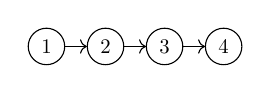
\begin{tikzpicture}[scale=0.75, every node/.style={transform shape}]
\graph[nodes={draw,circle}] {
1 -> 2 -> 3 -> 4
};
\end{tikzpicture}
 
\column{0.6\textwidth}

\begin{exampleblock}{}
\begin{minted}[fontsize=\footnotesize]{julia}
function foo!(A, b)
  @dspawn fill!(@W(b), 0)         # task 1
  @dspawn @RW(view(b, 1:2)) .+= 2 # task 2
  @dspawn @RW(view(b, 3:4)) .+= 3 # task 3
  @dspawn @R(A) \ @R(b)           # task 4
end
\end{minted}
\end{exampleblock}
\center 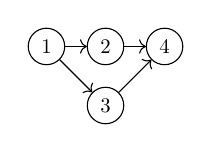
\begin{tikzpicture}[scale=0.75, every node/.style={transform shape}]
\graph[nodes={draw,circle}] {
  1 -> {2, 3} -> 4
};
\end{tikzpicture}

\end{columns}

% In this presentation, we will explore the features and benefits of \DFT{} in the context of efficient parallel programming.

\end{frame}

\begin{frame}
    \frametitle{Table of Contents}
    \tableofcontents
\end{frame}

\section{Introduction and high-level usage}

\subsection{Task based parallelism in Julia}

\begin{frame}[fragile]
\frametitle{Task based parallelism}
\begin{itemize}
    \item A task is a unit of execution or a unit of work
    \item \mintinline{julia}{Task} objects can be created using \mintinline{julia}{@task}
    \item Once created, \mintinline{julia}{Task} objects must be scheduled for execution
    \item Usually, \mintinline{julia}{Task}s are created + scheduled using \mintinline
    {julia}{@spawn}
    \item \alert{Responsibility of synchronizing tasks is left to the programmer}
\end{itemize}

\begin{columns}
\column{0.8\textwidth}    

\begin{example}[%
  \only<1>{Sequential}%
  \only<2>{Synchronizing tasks with return values}%
  \only<3>{Synchronizing tasks with explicit barriers}%
  ]
\begin{onlyenv}<1>
\begin{minted}[beameroverlays]{julia}
                   # Task
b = zeros(4)          # 1 - Initialization
b[1:2] .+= 2          # 2 - Work on first half
b[3:4] .+= 3          # 3 - Work on second half
res = A \ b           # 4 - Use entire vector
                      #
\end{minted}
\end{onlyenv}
\begin{onlyenv}<2>
\begin{minted}[beameroverlays]{julia}
                                         # Task
t1 = @spawn zeros(4)                        # 1
t2 = @spawn (b = fetch(t1); b[1:2] .+ 2)    # 2
t3 = @spawn (b = fetch(t1); b[3:4] .+ 3)    # 3
t4 = @spawn A \ vcat(fetch(t2), fetch(t3))  # 4
fetch(t4) # get result
\end{minted}
\end{onlyenv}
\begin{onlyenv}<3>
\begin{minted}[beameroverlays]{julia}    
b = Vector{Float64}(undef, 4)            # Task
t1 = @spawn fill!(b, 0)                     # 1
t2 = @spawn (wait(t1); view(b,1:2) += 2)    # 2
t3 = @spawn (wait(t1); view(b,3:4) += 3)    # 3
t4 = @spawn (wait(t2); wait(t3);  A \ b)    # 4
fetch(t4) # get result
\end{minted}
\end{onlyenv}
\end{example}

\column{0.15\textwidth}

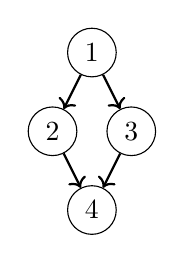
\begin{tikzpicture}
    % Nodes
    \node[circle, draw] (1) at (0, 0) {1};
    \node[circle, draw] (2) at (-0.5, -1) {2};
    \node[circle, draw] (3) at (0.5, -1) {3};
    \node[circle, draw] (4) at (0, -2) {4};
    % Edges
    \draw[->, thick] (1) -- (2);
    \draw[->, thick] (1) -- (3);
    \draw[->, thick] (2) -- (4);
    \draw[->, thick] (3) -- (4);
\end{tikzpicture}

\end{columns}

\end{frame}

\subsection{Motivation}

\begin{frame}[fragile]
\frametitle{Motivation for \texttt{DataFlowTasks}}

\begin{itemize}
    \item Reasoning about \mintinline{julia}{Task} interdependencies can be
    challenging
    \item Specially for algorithms making constant re-use of data   
    \item Sometimes, it is simpler to reason about how \mintinline{julia}{Task}s depend on data than how \mintinline{julia}{Task}s depend on each other
\end{itemize}

\begin{example}[Synchronizing tasks]
\begin{minted}[fontsize=\small]{julia}    
b = rand(4)
t1 = @spawn fill!(b,0)                   # RW access to b
t2 = @spawn (wait(t1); view(b,1:2) += 2) # RW access to b[1:2]
t3 = @spawn (wait(t1); view(b,3:4) += 3) # RW access to b[3:4]
t4 = @spawn (wait(t2); wait(t3);  A \ b) # R  access to A and b
fetch(t4)
\end{minted}
\end{example}

\begin{itemize}
  \item<2-> \alert{Would like to declare only the task-to-data dependencies}
\end{itemize}

\end{frame}

\subsection{Basic idea}

\begin{frame}[fragile]

\frametitle{Basic idea}
\begin{enumerate}
    \item \textcolor<4->{lightgray}{Extract data dependency from user annotations}
    \item \textcolor<1-3,10->{lightgray}{Infer task dependency from data dependency}
    \item \textcolor<1-9>{lightgray}{Schedule tasks with inferred dependencies}
\end{enumerate}

\center
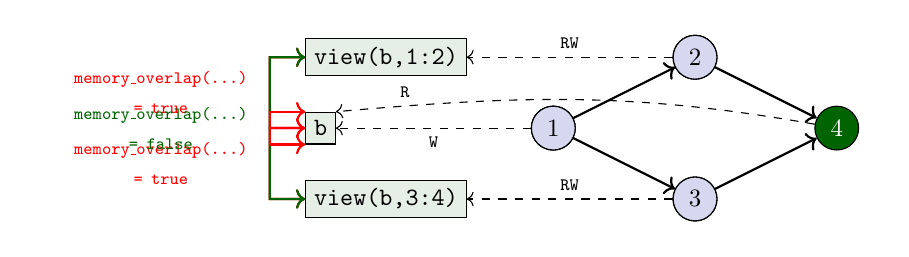
\begin{tikzpicture}[scale=0.9, every node/.style={transform shape}]
  % Tasks
  \node<2->[circle, draw] (1) at (0,  0) {1};
  \node<2>[circle, draw, fill=themegreen, text=white] at (0,  0) {1};
  \node<4,6,9>[circle, draw, fill=themelightblue] at (0,  0) {1};
  
  \node<3->[circle, draw] (2) at (2,  1) {2};
  \node<3-4>[circle, draw, fill=themegreen, text=white] at (2,  1) {2};
  \node<5,8>[circle, draw, fill=themelightblue] at (2,  1) {2};
  
  \node<5->[circle, draw] (3) at (2, -1) {3};
  \node<5-6>[circle, draw, fill=themegreen, text=white] at (2, -1) {3};
  \node<7>[circle, draw, fill=themelightblue] at (2, -1) {3};

  \node<7->[circle, draw, fill=themegreen, text=white] (4) at (4,  0) {4};
  
  % Data
  \node<1->[rectangle, draw, fill=themelightgreen, anchor=west] (A)  at (-3.5,  0) {\texttt{b}};
  \node<3->[rectangle, draw, fill=themelightgreen, anchor=west] (A1) at (-3.5,  1) {\texttt{view(b,1:2)}};
  \node<5->[rectangle, draw, fill=themelightgreen, anchor=west] (A2) at (-3.5, -1) {\texttt{view(b,3:4)}};
  
  % Task -> Data dependencies
  \draw<2->[->, dashed] (1) -- node[midway, below]{\scriptsize\ttfamily W} (A);
  \draw<3->[->, dashed] (2) -- node[midway, above]{\scriptsize\ttfamily RW} (A1) ;
  \draw<5->[->, dashed] (3) -- node[midway, above]{\scriptsize\ttfamily RW} (A2);
  \draw<7-> (4) edge[out=170, in=5, dashed, ->] node[pos=0.87, above]{\scriptsize\ttfamily R} (A.north east);
  
  % Task -> Task dependencies
  \draw<4->[->, thick] (1) -- (2);
  \draw<6->[->, thick] (1) -- (3);
  \draw<8->[->, thick] (2) -- (4);
  \draw<7->[->, thick] (3) -- (4);
  
  % Data <-> Data dependencies
  \draw<1-> (A.west)  ++(-0.5,0) node (Aw)  {};
  \draw<3-> (A1.west) ++(-0.5,0) node (A1w) {};
  \draw<5-> (A2.west) ++(-0.5,0) node (A2w) {};
  \draw<4,8>[<->, thick, red] (A.west)  -- (Aw.center)
  -- node[midway,left,text width=8em,align=center]{\scriptsize\ttfamily memory\_overlap(...) = true} (A1w.center) -- (A1.west);
  \draw<6,7>[<->, thick, red] (A.west)  -- (Aw.center)
  -- node[midway,left,text width=8em,align=center]{\scriptsize\ttfamily memory\_overlap(...) = true} (A2w.center) -- (A2.west);
  \draw<5>[<->, thick, themegreen] (A1.west) -- (A1w.center)
  -- node[midway,left,text width=8em,align=center]{\scriptsize\ttfamily memory\_overlap(...) = false} (A2w.center) -- (A2.west);
  \draw<9>[<->, thick, red] (A.south west) -- ++(-0.5,0) |- (A.north west);

  % Bounding box
  \node at (-7.3,-1.3) {};
  \node at (4.5,1.3) {};
\end{tikzpicture}

\begin{columns}[T]
  \column{0.42\textwidth}
\begin{exampleblock}{User-written code}
\begin{minted}[fontsize=\footnotesize,escapeinside=||,beameroverlays=true]{julia}
|\onslide<1->|b = rand(4)
|\onslide<2->|@dspawn fill!(@W(b),0)
|\onslide<3->|@dspawn @RW(view(b,1:2)) += 2
|\onslide<5->|@dspawn @RW(view(b,3:4)) += 3
|\onslide<7->|t4 = @dspawn A \ @R(b)
|\onslide<7->|fetch(t4)|\onslide<1->|
\end{minted}    
\end{exampleblock}
  
  \column{0.50\textwidth}
\begin{onlyenv}<4-9>
  \begin{exampleblock}{Behind the scenes: DAG}
\begin{minted}[fontsize=\footnotesize,escapeinside=||]{julia}
# Note the quadratic complexity!
for i in 1:N, j in i:-1:1
  # Detect conflict between i and j
  for di in data(i), dj in data(j)
    if memory_overlap(di, dj)
      add_edge(j, i)
\end{minted}
\end{exampleblock}
\end{onlyenv}
\begin{onlyenv}<10>
\begin{exampleblock}{Behind the scenes: task scheduling}
\begin{minted}[fontsize=\footnotesize]{julia}
t4 = Threads.@spawn begin
  wait(t2); wait(t3)
  A \ b
end
\end{minted}
\end{exampleblock}
\end{onlyenv}
\end{columns}

% \alert{Note the quadratic complexity in the number of tasks!}

\end{frame}

% \subsection{Simple example: parallel merge sort}

% \begin{frame}
% \frametitle{Simple example}
% \center \href{run:./sort.slides.html}{\LARGE{Demo: parallel merge sort}}

% \end{frame}


\section{Real use case: tiled Cholesky}

\subsection{Algorithm}

\begin{frame}{Tiled Cholesky factorization: idea}
  \begin{itemize}
  \item Objective: take a SPD matrix $A$, find lower triangular $L$ such
    that \[A=LL^\top\]
  \item Idea for a tiled algorithm:
    \begin{align*}
      \begin{bmatrix}
        A_{11} & A_{12} \\
        A_{12}^\top & A_{22}
      \end{bmatrix} = 
      \textcolor{gray}{
      \begin{bmatrix}
        \textcolor<2->{black}{L_{11}} & \\
        \textcolor<3->{black}{L_{21}} & \textcolor<4->{black}{L_{22}}
      \end{bmatrix}
      \begin{bmatrix}
        \textcolor<2->{black}{L^\top_{11}} & \textcolor<3->{black}{L^\top_{21}} \\
        & \textcolor<4->{black}{L^\top_{22}}
      \end{bmatrix}
      }
    \end{align*}
    \vspace{-10pt}
    \begin{enumerate}
    \item<2-> $A_{11} = L_{11} L^\top_{11}$\\
      $\vartriangleright$ Cholesky factorization to get $L_{11}$\hfill\texttt{cholesky!}\medskip
    \item<3-> $A_{12} = L_{11} L^\top_{21}$\\
      $\vartriangleright$ Triangular solve to get $L_{21}$\hfill\texttt{ldiv!}\medskip
    \item<4-> $A_{22} - L_{21} L^\top_{21} = L_{22} L^\top_{22}$\\
      $\vartriangleright$ Matmul to get $A_{22} - L_{21} L^\top_{21}$\hfill\texttt{mul!}\\
      $\vartriangleright$ Cholesky factorization to get $L_{22}$\hfill\texttt{cholesky!}
    \end{enumerate}
  \end{itemize}
\end{frame}


\begin{frame}
  \frametitle{Tiled Cholesky factorization: algorithm}
  \begin{itemize}
    \item Input: symmetric positive-definite matrix $A$ with $N \times N$ blocks
    \item Goal: compute lower-triangular $L$ such that $A = L L^\top$
  \end{itemize}

  \bigskip  

  \begin{columns}
    \column{0.45\textwidth}
    \centering 
\begin{tikzpicture}[thick, scale=1, transform shape]
      \foreach \y in {1,2,...,4}  {
        \foreach \x in {1,2,...,4} {
          % fill with blue if above diagonal, with white otherwise
          \pic[fill=blue!50] at (\x,\y) {square};
        }
      }
      % fill blocks below main diagonal with white
      \pic[fill=white] at (2,4) {square};
      \pic[fill=white] at (3,3) {square};
      \pic[fill=white] at (3,4) {square};
      \pic[fill=white] at (4,4) {square};
      \pic[fill=white] at (4,3) {square};
      \pic[fill=white] at (4,2) {square};

      % diagonal 1,1
      \only<2,3,4>{\pic[fill=themegreen] at (1,4) {square};}
      \only<3,4>{
        % first row
        \pic[fill=orange] at (1,3) {square};
        \pic[fill=orange] at (1,2) {square};
        \pic[fill=orange] at (1,1) {square};
      }
      % draw an arrow from (1,4) to (2,4), (3,4) and (4,4)
      \only<3>{
        \draw[->, thick, gray!30] (1.25,4.5) -- (1.25,3.5);
        \draw[->, thick, gray!30] (1.5,4.5) -- (1.5,2.5);
        \draw[->, thick, gray!30] (1.75,4.5) -- (1.75,1.5);
      }
      % fill blocks below diagonal 1,1 in green
      \only<4>{
      \pic[fill=red] at (2,1) {square};
      \pic[fill=red] at (2,2) {square};
      \pic[fill=red] at (2,3) {square};
      \pic[fill=red] at (3,1) {square};
      \pic[fill=red] at (3,2) {square};
      \pic[fill=red] at (4,1) {square};
      }
      % draw arrows from first row into green blocks
      \only<4>{
        \draw[->, thick, gray!30] (1.5,3.5) -- (2.5,3.5);
        \draw[->, thick, gray!30] (1.5,2.625) -- (2.5,2.625);
        \draw[->, thick, gray!30] (1.5,2.375) -- (3.5,2.375);
        \draw[->, thick, gray!30] (1.5,1.75) -- (2.5,1.75);
        \draw[->, thick, gray!30] (1.5,1.5) -- (3.5,1.5);
        \draw[->, thick, gray!30] (1.5,1.25) -- (4.5,1.25);
      }
      \only<5->{
        % start the next iteration
        \pic[fill=gray!30] at (1,1) {square};
        \pic[fill=gray!30] at (1,2) {square};
        \pic[fill=gray!30] at (1,3) {square};
        \pic[fill=gray!30] at (1,4) {square};
      }
      \only<6->{
        % fill whole matrix with gray
        \pic[fill=gray!30] at (2,1) {square};
        \pic[fill=gray!30] at (2,2) {square};
        \pic[fill=gray!30] at (2,3) {square};
        \pic[fill=gray!30] at (3,1) {square};
        \pic[fill=gray!30] at (3,2) {square};
        \pic[fill=gray!30] at (4,1) {square};
      }
   \end{tikzpicture}

   \medskip   
   \center \only<2-4>{\texttt{i=1}}
   \center \only<5>{\texttt{i=2}, repeat}
    
    \column{0.55\textwidth}
    \only<2->{\texttt{for i in 1:N}}
    \begin{enumerate}
      % cholesky in themegreen
      \item<2-> \textcolor{themegreen}{\texttt{cholesky!}} \\
      $A_{i,i} \leftarrow \texttt{chol!}(A_{i,i})$ \\
      $L_{i,i} = \texttt{LowerTriangular}(A_{i,i})$
      \item<3-> \textcolor{orange}{\texttt{ldiv!}} \\
      \texttt{for k in 2:N}\\
      \quad $A_{k,i} \leftarrow \texttt{ldiv!}(L_{i,i}, A_{k,i}),$
      \item<4-> \textcolor{red}{\texttt{mul!}} \\
      \texttt{for k in i+1:N, j in i+1:k}\\
      \quad $A_{k,j} \leftarrow A_{k,j} - A_{k,i}A^\top_{k,i}$
    \end{enumerate}
  \end{columns}
  
  \bigskip
  \begin{itemize}  
    \item<6-> Output: $L$ in the lower-triangular part of $A$
  \end{itemize}

\end{frame}

\begin{frame}
  \frametitle{Tiled Cholesky factorization: complexity}

  \begin{columns}[T]
    \column{0.45\textwidth}
    \centering 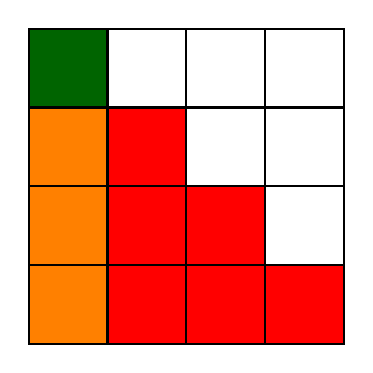
\begin{tikzpicture}[thick, scale=1, transform shape]
      \foreach \x in {1,2,...,4}  {
        \foreach \y in {1,2,...,4} {
          % fill with blue if above diagonal, with white otherwise
          \pic[fill=blue!50] at (\x,\y) {square};
        }
      }
      % fill blocks below main diagonal with white
      \pic[fill=white] at (2,4) {square};
      \pic[fill=white] at (3,3) {square};
      \pic[fill=white] at (3,4) {square};
      \pic[fill=white] at (4,4) {square};
      \pic[fill=white] at (4,3) {square};
      \pic[fill=white] at (4,2) {square};

      % diagonal 1,1
      \pic[fill=themegreen] at (1,4) {square};
      % first col
      \pic[fill=orange] at (1,3) {square};
      \pic[fill=orange] at (1,2) {square};
      \pic[fill=orange] at (1,1) {square};
      % draw an arrow from (1,4) to (2,4), (3,4) and (4,4)
      % \draw[|->, thick] (1.5,4.75) -- (2.5,4.75);
      % \draw[|->, thick] (1.5,4.5) -- (3.5,4.5);
      % \draw[|->, thick] (1.5,4.25) -- (4.5,4.25);
      % fill blocks below diagonal 1,1 in green
      \pic[fill=red] at (2,1) {square};
      \pic[fill=red] at (2,2) {square};
      \pic[fill=red] at (2,3) {square};
      \pic[fill=red] at (3,1) {square};
      \pic[fill=red] at (3,2) {square};
      \pic[fill=red] at (4,1) {square};
      % % draw arrows from first row into green blocks
      % \draw[|->, thick] (2.5,4.5) -- (2.5,3.5);
      % \draw[|->, thick] (3.375,4.5) -- (3.375,3.5);
      % \draw[|->, thick] (3.625,4.5) -- (3.625,2.5);
      % \draw[|->, thick] (4.25,4.5) -- (4.25,3.5);
      % \draw[|->, thick] (4.5,4.5) -- (4.5,2.5);
      % \draw[|->, thick] (4.75,4.5) -- (4.75,1.5);
   \end{tikzpicture}
    \column{0.55\textwidth}
    % \begin{onlyenv}<1>
    %   $N$ steps for an $N \times N$ block matrix;\\
    %   each step $i$ performs:
    %   \begin{itemize}
    %   \item $1$ Cholesky factorization of the $(i,i)$ tile,
    %   \item $(i-1)$ triangular solves (one for each tile in the $i$-th row of the upper triangular matrix),
    %   \item $i(i-1)/2$ matrix multiplications to update the submatrix.
    %   \end{itemize}
    % \end{onlyenv}
    \begin{onlyenv}<1>
      For an $N \times N$ block matrix:\\
      \begin{itemize}
      \item $\mathcal{O}(N)$ \textcolor{themegreen}{cholesky factorizations}
      \item $\mathcal{O}(N^2)$ \textcolor{orange}{triangular solves}
      \item $\mathcal{O}(N^3)$ \textcolor{red}{matrix multiplications}
        \medskip
      \end{itemize}
      Globally compute-bound:
      \begin{itemize}
      \item $\mathcal{O}(N^3)$ flops for
      \item $\mathcal{O}(N^2)$ bytes
      \item[$\Rightarrow$] potential for efficient parallelism
      \end{itemize}
    \end{onlyenv}
  \end{columns}
\end{frame}

\subsection{Sequential \& parallel implementation}

\begin{frame}[fragile]{Tiled Cholesky factorization: sequential implementation}
  \begin{minted}[fontsize=\scriptsize]{julia}
function cholesky_tiled!(A, ts)
  m = size(A, 1); n = m ÷ ts      # Matrix size & number of tiles
  T = [view(A, tilerange(i, ts), tilerange(j, ts)) for i in 1:n, j in 1:n]

  for i in 1:n
    cholesky!(T[i,i])             # Diagonal cholesky serial factorization

    U = UpperTriangular(T[i,i])   # Left tiles update
    for j in i+1:n
      ldiv!(U', T[i,j])
    end

    for j in i+1:n, k in j:n      # Submatrix update
      mul!(T[j,k], T[i,j]', T[i,k], -1, 1)
    end
  end

  # Construct the factorized object
  return Cholesky(A, 'U', zero(LinearAlgebra.BlasInt))
end
  
  \end{minted}
\end{frame}


\begin{frame}[fragile]{Tiled Cholesky factorization: parallel implementation}
  \begin{minted}[fontsize=\scriptsize]{julia}
function cholesky_dft!(A, ts)
  m = size(A, 1); n = m ÷ ts      # Matrix size & number of tiles
  T = [view(A, tilerange(i, ts), tilerange(j, ts)) for i in 1:n, j in 1:n]

  for i in 1:n
    @dspawn cholesky!(@RW(T[i,i]))    label="chol ($i,$i)"

    U = UpperTriangular(T[i,i])
    for j in i+1:n
      @dspawn ldiv!(@R(U)', @RW(T[i,j]))    label="ldiv ($i,$j)"
    end

    for j in i+1:n, k in j:n
      @dspawn mul!(@RW(T[j,k]),@R(T[i,j])',@R(T[i,k]),-1, 1) label="schur($j,$k)"
    end
  end

  # Construct the factorized object
  r = @dspawn Cholesky(@R(A), 'U', zero(LinearAlgebra.BlasInt)) label="result"
  return fetch(r)
end 
  \end{minted}
\end{frame}

\begin{frame}[fragile]{Tiled Cholesky factorization: performance}
\begin{minted}[fontsize=\footnotesize]{jlcon}
julia> using BenchmarkTools

julia> n = 4096; ts = 512;

julia> t_seq = @belapsed(cholesky_tiled!(A, ts),
                         setup=(A=spd_matrix(n)), evals=1)
0.559141485

julia> t_par = @belapsed(cholesky_dft!(A, ts),
                         setup=(A=spd_matrix(n)), evals=1)
0.108479304

julia> (; threads = Threads.nthreads(),
          speedup = t_seq / t_par)
(threads = 8, speedup = 5.15436089063056)
\end{minted}
\end{frame}

\subsection{Profiling \& debugging tools}

\begin{frame}[fragile]{Tiled Cholesky factorization: profiling \& debugging}
  \begin{minted}[fontsize=\footnotesize]{jlcon}
julia> n = 4096; ts = 512;
    
julia> A = spd_matrix(n);
    
julia> log_info = DataFlowTasks.@log cholesky_dft!(Ac, ts)
LogInfo with 121 logged tasks

julia> DataFlowTasks.describe(log_info;categories=["chol","ldiv","schur"])
• Elapsed time           : 0.297
  +  Critical Path       : 0.253
  +  No-Wait             : 0.188

• Run time               : 2.379
  +  Computing           :   1.507
     o  chol             :     0.061
     o  ldiv             :     0.414
     o  schur            :     1.032
     o  unlabeled        :     0.000
  +  Task Insertion      :   0.003
  +  Other (idle)        :   0.870
\end{minted}
\end{frame}

\begin{frame}[fragile]{Tiled Cholesky factorization: profiling \& debugging}
\begin{minted}[fontsize=\footnotesize]{jlcon}
julia> DataFlowTasks.stack_weakdeps_env!()
julia> using GraphViz
[ Info: Loading DataFlowTasks dag plot utilities
julia> GraphViz.Graph(log_info)
\end{minted}
\includegraphics[width=\textwidth]{Cholesky_dag.png}
\end{frame}

\begin{frame}[fragile]{Tiled Cholesky factorization: profiling \& debugging}
\begin{minted}[fontsize=\footnotesize]{jlcon}
julia> using CairoMakie # or GLMakie for more interactivity
[ Info: Loading DataFlowTasks profile plot utilities
julia> plot(log_info; categories=["chol", "ldiv", "schur"])
\end{minted}
\includegraphics[width=\textwidth]{Cholesky_profile.png}

\end{frame}

\subsection{Comparison to OpenBLAS}

\begin{frame}{Comparison to openBLAS}
  \center \Large How does it compare to multi-threaded OpenBLAS?
\end{frame}

\begin{frame}{Tiled Cholesky factorization: performance}
  \centering\includegraphics[width=0.92\textwidth]{Cholesky_perf.png}
\end{frame}

\begin{frame}{Tiled Cholesky factorization: performance}
  \centering\includegraphics[width=0.92\textwidth]{traceplot_large.png}
\end{frame}
  
% Focus on the cholesky example for the remainder of the talk (say to 10 to 15 minutes). IMO it should include:

%     why this example is a good benchmark (e.g. a good arithmetic intensity since you do $n^3$ flops for $n^2$ bytes, so you can expect to gain from "good" parallelism since you are compute-bound). For some of the other examples we have in the docs we are most likely memory-bound.
%     A discussion of the tiled algorithm. It is not hard, but we need to show where it comes from. I would map each operation to the corresponding julia function at some point (e.g. mul!, cholesky!, ldiv!). Discuss that we call OpenBLAS for simplicity, but having those kernels efficiently done in julia is relatively simple if one uses LoopVectorization.
%     Then show how to parallelize it using DFT
%     Explore the @log information, and how to read/interpret it
%     Comparison to OpenBLAS



\section{Concluding remarks}

% \begin{frame}
% \frametitle{Summary}  

% \begin{itemize}
%   \item When \DFT{} is loaded a default \mintinline{julia}{TaskGraph}, with an
%   internal \mintinline{julia}{DAG}, is instantiated.
%   \item Upon creation, each \mintinline{julia}{DataFlowTask} object inserts
%   itself in the task graph.
%   \item Upon completion, each \mintinline{julia}{DataFlowTask} object inserts
%   itself in a finished channel
%   \item An asynchronous task is responsible for removing finished jobs from the graph
%   \item The \mintinline{julia}{@dspawn} macro provides a very convenient way to
%   create \mintinline{julia}{DataFlowTask}s
%   \item Logging is enabled using the \mintinline{julia}{@log} macro
% \end{itemize} 
% \end{frame}

\begin{frame}
\frametitle{Concluding remarks}

\begin{itemize}
  \item \DFT{} tries to make parallel programming easier for \emph{certain types of algorithms}
  \item Simple API: \mintinline{julia}{@dspawn} macro
  \item Several supplementary examples in the online documentation
\end{itemize} 

\bigskip

\begin{block}{}
  \center {\large \url{https://github.com/maltezfaria/DataFlowTasks.jl}}
\end{block}

\bigskip

\center If you think \DFT{} may help parallelize your algorithm, please give it
a try or reach out to us!

\end{frame}

\appendix

\begin{frame}
  \begin{center}
    \Huge Appendix
  \end{center}
\end{frame}

\section{\mintinline{julia}{Implementation details}}

\begin{frame}{Main types}

The package revolves around three main types:
\begin{itemize}
  \item <1->\mintinline{julia}{DataFlowTask}: wrapper around a
  \mintinline{julia}{Task} with user-declared data dependencies
  \item <2->\mintinline{julia}{DAG}: graph data
  structure to represent dependencies between \mintinline{julia}{DataFlowTask}s
  \item <3->\mintinline{julia}{TaskGraph}: a
  \mintinline{julia}{DAG} and some helper functions/workers to manage it

\end{itemize}

\begin{alertblock}<4->{}
  Next: some technical details about their
  implementation.
\end{alertblock}

\end{frame}

\subsection{\mintinline{julia}{DataFlowTask}}

\begin{frame}[fragile]

\frametitle{\texttt{DataFlowTask}: \mintinline{julia}{@dspawn} macro}

\texttt{DataFlowTask}s are created using \mintinline{julia}{@dspawn}. The macro
does the following:

\begin{itemize}
    \item Scan the \mintinline{julia}{Expr} for \mintinline{julia}{@R, @W, @RW} annotations
    \item Create a \mintinline{julia}{data} and \mintinline{julia}{mode}
    tuples
    \item Remove annotations from the \mintinline{julia}{Expr}
    \item Parse keyword arguments    
    \item Create an anonymous function wrapping the new \mintinline{julia}{Expr}
    \item Insert a call to \mintinline{julia}{DataFlowTask} constructor
\end{itemize}

\begin{columns}

\column{0.45\textwidth}    
\begin{exampleblock}{User-written code}    
\begin{minted}{julia}
@dspawn(foo!(@W(B), @R(A)),
        label="foo!")
\end{minted}
\end{exampleblock}

\column{0.45\textwidth}    

\begin{exampleblock}{Macro expansion (approx.)}
\begin{minted}{julia}
_t = DataFlowTask(
       () -> foo!(B, A),
       (B, A),
       (WRITE, READ);
       label="foo!")
spawn(_t)
\end{minted}
\end{exampleblock}

\end{columns}
%

\end{frame} 

\begin{frame}[fragile]

\frametitle{\texttt{DataFlowTask} structure}

\small{\alert{Inner-constructor of \mintinline{julia}{DataFlowTask} handles much of
the insertion/removal logic:}}

\hrulefill
\begin{minted}[fontsize=\footnotesize]{julia}
mutable struct DataFlowTask
  data::Tuple
  access_mode::NTuple{<:Any,AccessMode}
  task::Task
  ...
  function DataFlowTask(f,data,mode,taskgraph)
    tj = new(data, mode) # incomplete initialization
    addnode!(taskgraph, tj, true) 
    deps = inneighbors(taskgraph, tj) |> copy
    tj.task = @task do
      foreach(wait,deps)
      res = f() # run the underlying function
      put!(taskgraph.finished, tj)
      return res
    end
  end
end
\end{minted}

\end{frame} 

\subsection{\mintinline{julia}{DAG}}

\begin{frame}[fragile]
\frametitle{{\mintinline{julia}{DAG}}}  

Graph structure used to represent dependencies between \mintinline{julia}{DataFlowTask}s:

\begin{itemize}
  \item Dynamic: nodes are added and removed on the fly
  \item \textbf<2>{Buffered: limit the number of active nodes}
  \item \textbf<3>{Thread-safe: multiple threads can add/remove nodes}
  \item Efficient: easy access to both in- and out-neighbors
\end{itemize}

\hrulefill

\begin{columns}

\column{0.45\textwidth}
\begin{exampleblock}{}
\begin{minted}[fontsize=\footnotesize]{julia}
struct DAG{T}
  inoutlist::OrderedDict{...}
  cond_push::Condition
  lock::ReentrantLock
  sz_max::Base.RefValue{Int}
  ...
end
\end{minted}
\end{exampleblock}

\column{0.55\textwidth}

\begin{onlyenv}<2>
\begin{itemize}
  \item[$\triangleright$] \mintinline{julia}{addnode!(dag,node)} calls
  \mintinline{julia}{wait(cond_push)} if full
  \item[$\triangleright$] \mintinline{julia}{removenode!(dag,node)} calls \mintinline{julia}{notify(cond_push)}
\end{itemize}
\end{onlyenv}

\begin{onlyenv}<3>
  \begin{itemize}
    \item[$\triangleright$] mutating the \texttt{DAG} requires acquiring/releasing the \texttt{lock}
    \item[$\triangleright$] pattern: \mintinline{julia}{@lock dag.lock code}
  \end{itemize}
  \end{onlyenv}


\end{columns}

\end{frame}

\subsection{\mintinline{julia}{TaskGraph}}

\begin{frame}[fragile]
\frametitle{{\mintinline{julia}{Taskgraph}}}  
  
Essentially a \mintinline{julia}{DAG{DataFlowTask}} with
\begin{itemize}
  \item A channel to store finished tasks  
  \item A dedicated \mintinline{julia}{Task} to remove nodes from the graph
\end{itemize}

\hrulefill

\begin{columns}

\column{0.45\textwidth}
\begin{minted}[fontsize=\footnotesize]{julia}
mutable struct TaskGraph
  dag::DAG{DataFlowTask}
  finished::FinishedChannel
  dag_cleaner::Task
  function TaskGraph(sz)
    dag = DAG{DataFlowTask}(sz)
    finished = FinishedChannel()
    tg = new(dag, finished)
    start_dag_cleaner(tg)
    return tg
  end
end
\end{minted}

\column{0.5\textwidth}
\begin{itemize}
  \item[$\triangleright$] Insertion done by \mintinline{julia}{DataFlowTask} constructor
  \item[$\triangleright$] Removal done in two steps:
  \begin{enumerate}
    \item The \mintinline{julia}{node.task} moves the node into the finished channel
    \item Dedicated task handles finished channel
  \end{enumerate}
\end{itemize}  

\end{columns}

\end{frame}

\subsection{Logging}

\begin{frame}
\frametitle{Logging}

Some logging capabilities available:
\begin{itemize}
  \item \mintinline{julia}{@log} macro logs the execution of block
  \item \mintinline{julia}{describe(loginfo)} shows a summary
  \item \mintinline{julia}{Graph(loginfo)} displays the \mintinline{julia}{DAG}
  \item \mintinline{julia}{plot(loginfo)} plots the execution trace
\end{itemize}

\end{frame}

\begin{frame}[fragile]
\frametitle{Logging}

Basic idea:
\begin{itemize}
  \item Redefine the function
  \mintinline{julia}{should_log()} to control logging
  \item Tasks conditionally create a \mintinline{julia}{TaskLog} object
  \item Information dumped into \mintinline{julia}{LogInfo} object
  \item Logging should have zero overhead when disabled
\end{itemize}

\hrulefill

\begin{columns}

\column{0.45\textwidth}  

\begin{minted}[fontsize=\footnotesize]{julia}
struct TaskLog
  tag::Int
  time_start::UInt64
  time_finish::UInt64
  tid::Int
  inneighbors::Vector{Int64}
  label::String
end
\end{minted}

\column{0.45\textwidth}  

Known limitations:
\begin{itemize}
  \item[$\triangleright$] If the function \mintinline{julia}{yield}s, logged task time is
  not representative of execution time
\end{itemize}

\end{columns}

\end{frame}

\begin{frame}{Tiled Cholesky factorization: performance}
  \centering\includegraphics[width=0.92\textwidth]{openblas_large.png}
\end{frame}
\begin{frame}{Tiled Cholesky factorization: performance}
  \centering\includegraphics[width=0.92\textwidth]{perf_large.png}
\end{frame}
  
  \begin{frame}{Tiled Cholesky factorization: performance}
    \centering\includegraphics[width=0.92\textwidth]{trace_with_gc.png}
\end{frame}

% \begin{frame}[fragile]
% \frametitle{Logging}

% \begin{minted}[fontsize=\footnotesize]{julia}
% function work(A, B)
%     @dspawn init!(@W(A))               label="init A"
%     @dspawn init!(@W(B))               label="init B"
%     @dspawn mutate!(@RW(A))            label="mutate A"
%     @dspawn mutate!(@RW(B))            label="mutate B"
%     res = @dspawn result(@R(A), @R(B)) label="read A,B"
%     fetch(res)
% end
% log_info = DataFlowTasks.@log work(A, B)
% DataFlowTasks.describe(log_info; categories=["init", "mutate", "read"])

% \end{minted}

% \center \includegraphics[width=0.3\textwidth]{figures/unicode-output.png}
  
% \end{frame}

% \begin{frame}[fragile]
% \frametitle{Logging}

% \begin{minted}[fontsize=\footnotesize]{julia}
% function work(A, B)
%   @dspawn init!(@W(A))               label="init A"
%   @dspawn init!(@W(B))               label="init B"
%   @dspawn mutate!(@RW(A))            label="mutate A"
%   @dspawn mutate!(@RW(B))            label="mutate B"
%   res = @dspawn result(@R(A), @R(B)) label="read A,B"
%   fetch(res)
% end
% using GraphViz
% GraphViz.Graph(log_info)
  
% \end{minted}
  
% \center \includegraphics[width=0.3\textwidth]{figures/dag-output.png}
    
% \end{frame}

% \begin{frame}[fragile]
% \frametitle{Logging}

% \begin{minted}[fontsize=\footnotesize]{julia}
% function work(A, B)
%   @dspawn init!(@W(A))               label="init A"
%   @dspawn init!(@W(B))               label="init B"
%   @dspawn mutate!(@RW(A))            label="mutate A"
%   @dspawn mutate!(@RW(B))            label="mutate B"
%   res = @dspawn result(@R(A), @R(B)) label="read A,B"
%   fetch(res)
% end
% using CairoMakie # or GLMakie to benefit from more interactivity
% plot(log_info; categories=["init", "mutate", "read"])
    
%   \end{minted}
    
%   \center \includegraphics[width=0.8\textwidth]{figures/trace-output.png}
      
%   \end{frame}

\end{document}